% ============================================================================
% Paste-ready Model V section for the MAT3300 report (Question 4:
% "Does similarity data support that the identified influencers actually
% influence the respective artists? Are some characteristics more
% contagious than others?")
%
% Requirements in the main document:
%   * figures/feature_contagion_excess.pdf   (fig11)
%   * figures/dose_response_excess.pdf       (fig12)
%   * booktabs, amsmath, graphicx, cleveref (already in the preamble)
% Labels follow the team convention: subsec:q4-*, eq:q4-*, fig:q4-*, tab:q4-*.
% ============================================================================

\section{Model IV: Does Influence Leave an Acoustic Trace?}\label{sec:model-q4}

The last question of Problem~C asks whether the similarity data actually
\emph{support} the influence relationships reported in
\texttt{influence\_data.csv}: do the ``influencers'' genuinely shape the
music of their followers, and are some musical characteristics more
\emph{contagious} than others? Model~II measures how similar two artists
sound; Model~I records \emph{who claimed to influence whom}. Neither
alone answers the question, because a high similarity along a reported
edge may simply reflect \emph{homophily}---followers choose their
influencers from artists they already sound like. This section therefore
combines the two models in a matched-control design: the reported edges
of Model~I are the treatment group, and statistically comparable
\emph{unrelated} artist pairs form the control group, so that any
excess resemblance along the edges can be attributed to the reported
influence rather than to selection.

\subsection{Matched-Control Excess Similarity}\label{subsec:q4-design}

Let $s(i,j)=1/(1+\lVert\tilde{\mathbf{x}}_i-\tilde{\mathbf{x}}_j\rVert_2)$
be the bounded similarity of Model~II in the global $z$-space
(\cref{subsec:q3-centroids}). For every reported edge $(i,j)$ of
Model~I we draw $K=10$ \emph{control} artists $j'$ matched to $j$ on the
two variables that drive homophily---main genre $\mathcal{G}(j')=
\mathcal{G}(j)$ and active-start decade $t(j')=t(j)$---with the
constraint that no edge $(i,j')$ exists in the influence data. The
\emph{excess similarity} of the edge is
\begin{equation}\label{eq:q4-excess}
s^{*}(i,j)=s(i,j)-\frac{1}{K}\sum_{k=1}^{K}s(i,j'_k),
\end{equation}
the resemblance along the edge beyond what the genre-and-decade baseline
predicts. A positive and significant $s^{*}$ means the follower's sound
is closer to the influencer than to comparable artists they did
\emph{not} choose---evidence \emph{consistent with} influence (the data
provide a single post-hoc snapshot per artist, so the design supports
consistency claims, not before/after causal proof; we use this wording
throughout).

All $42{,}770$ edges enter the test except $18$ edges whose endpoints
lack audio features and $55$ edges whose follower-genre/decade cell
contains no admissible control ($42{,}697$ edges analysed; the dropped
$0.17\%$ are disclosed rather than imputed). Features, standardization
and similarity are inherited from Model~II without modification, and the
edge table and decade convention are those of Model~I
(Assumption~A2); no new parameter enters except the control count $K$,
whose variation is discussed in the robustness paragraph.

\subsection{Do Influencers Actually Shape Their Followers?}\label{subsec:q4-overall}

The edges are systematically more similar than their controls: mean edge
similarity $0.286$ versus $0.250$ along matched controls, giving
$\bar{s}^{*}=0.0354$ with a bootstrap $95\%$ confidence interval
$[0.0347,\,0.0360]$ and a one-sided Wilcoxon $p<10^{-15}$;
$70.1\%$ of individual edges have $s^{*}>0$. The effect is modest in
absolute size---homophily explains most of the raw resemblance, as the
control construction makes visible---but it is extremely consistent:
reported influence carries a genuine acoustic signature that survives
matching on genre and era. We conclude that the similarity data
\emph{do} support the reported influence network.

\subsection{Which Characteristics Are Contagious?}\label{subsec:q4-features}

Repeating the matched-control comparison coordinate by coordinate
yields a per-feature excess
$a_f=\mathbb{E}[\,|\tilde{x}_j^{f}-\tilde{x}_{i}^{f}|\,]\text{ control minus edge}$,
reported in \cref{tab:q4-features} and \cref{fig:q4-features}.
The answer to ``are all characteristics equally contagious'' is a clear
\emph{no}: the gradient spans a factor of six. Style-defining
characteristics dominate---acousticness, valence, energy and
danceability all show excesses around $0.15$ in median
$z$-units---whereas technical or structural characteristics
(instrumentalness, speechiness, duration) show excesses an order of
magnitude smaller. Loudness and tempo occupy the middle ground. In
other words, followers absorb \emph{how the music feels} (texture,
mood, groove) far more reliably than \emph{how it is organised}.

The magnitude-versus-median contrast also flags distributional caveats:
instrumentalness has mean excess $0.121$ but median excess $0.027$,
i.e.\ its apparent contagion is driven by a heavy tail of extreme
values; medians are therefore our headline statistic.

\begin{table}[htbp]
\centering\small
\begin{tabular}{lrrrr}
\toprule
feature & excess mean & excess median & $\beta_f$ (edges) & $\beta_f$ (controls) \\
\midrule
acousticness    & 0.172 & \textbf{0.169} & $-0.000$ & $-0.007$ \\
valence         & 0.165 & \textbf{0.155} & $0.119$  & $-0.004$ \\
energy          & 0.179 & \textbf{0.154} & $-0.026$ & $-0.002$ \\
danceability    & 0.173 & \textbf{0.146} & $0.272$  & $0.000$ \\
tempo           & 0.125 & 0.110          & $-0.054$ & $-0.004$ \\
loudness        & 0.090 & 0.064          & $-0.000$ & $0.003$ \\
popularity      & 0.062 & 0.049          & $0.036$  & $-0.003$ \\
liveness        & 0.071 & 0.047          & $-0.014$ & $-0.001$ \\
duration\_ms    & 0.069 & 0.044          & $-0.014$ & $0.009$ \\
speechiness     & 0.085 & 0.034          & $0.023$  & $0.006$ \\
instrumentalness& 0.121 & 0.027          & $-0.045$ & $0.000$ \\
\bottomrule
\end{tabular}
\caption{Per-feature contagion. Excess alignment
$a_f$ (control minus edge absolute difference in $z$-units) and
directional regression coefficients
$x_j^{f}=\beta_f x_i^{f}+\text{genre FE}+\text{decade FE}+\varepsilon$
fitted separately on reported edges and on pooled matched-control
pairs. Bold medians mark the four highly contagious characteristics.}
\label{tab:q4-features}
\end{table}

\begin{figure}[htbp]
\centering
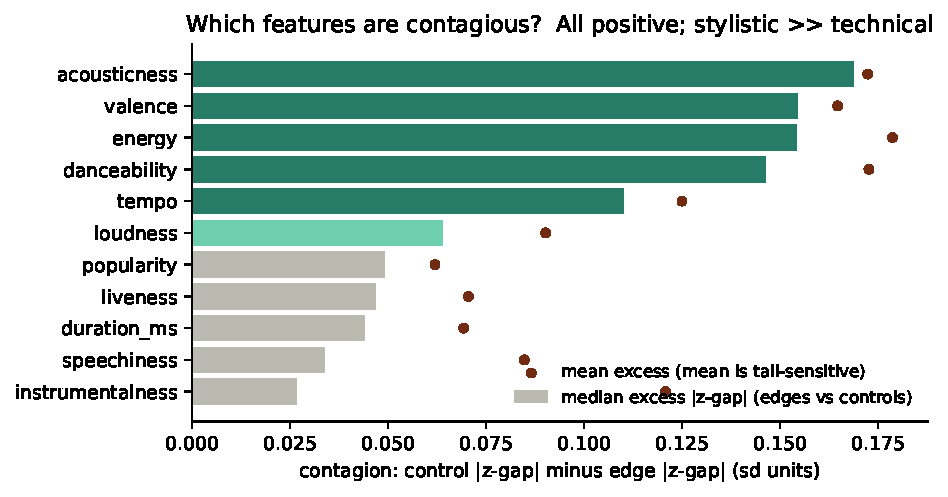
\includegraphics[width=0.9\textwidth]{feature_contagion_excess.pdf}
\caption{Contagion of musical characteristics: median (dark) and mean
(light) matched-control excess alignment per feature. Style
characteristics (acousticness, valence, energy, danceability) are
contagious; structural characteristics (instrumentalness, speechiness,
duration) are not.}
\label{fig:q4-features}
\end{figure}

\paragraph{Directional regression.}
Magnitude contagion does not imply \emph{directional} tracking. Fitting
$x_j^{f}=\beta_f x_i^{f}+\text{FE}+\varepsilon$ on the edges
(\cref{tab:q4-features}, columns 4--5), only \texttt{danceability}
($\beta=0.272$ versus $0.000$ on controls) and \texttt{valence}
($0.119$) show a clear ``influencer high $\Rightarrow$ follower high''
pull, while \texttt{energy}---strongly contagious in magnitude---has
$\beta\approx-0.03$. The divergence between $a_f$ and $\beta_f$ has a
natural reading: the average follower reports ${\sim}7.6$ influencers,
so a follower's coordinate is a mixture of many sources and random
dips; edges then show compressed \emph{distances} without linear
\emph{tracking}. Magnitude contagion and directional contagion are
different phenomena, and only danceability and valence pass both tests.

\subsection{Influence Strength versus Acoustic Trace}\label{subsec:q4-dose}

If reported influence were purely acoustic imitation, strongly
influential artists should leave stronger traces. The data show the
opposite. Binning edges by the influencer's outgoing Katz score of
Model~I (\cref{fig:q4-dose}, left), mean excess similarity declines
monotonically above the median: $0.040$ in the second Katz quintile
versus $0.028$ in the top quintile (Spearman
$\rho=-0.032$, $p<10^{-10}$ over edges). Highly influential artists are
cited \emph{beyond} what their sound predicts---a status component of
influence---whereas weaker influencers are cited precisely because
their sound is imitated. This complements Model~I, where edge counts
already separated reported prestige from network-transmitted influence.

\begin{figure}[htbp]
\centering
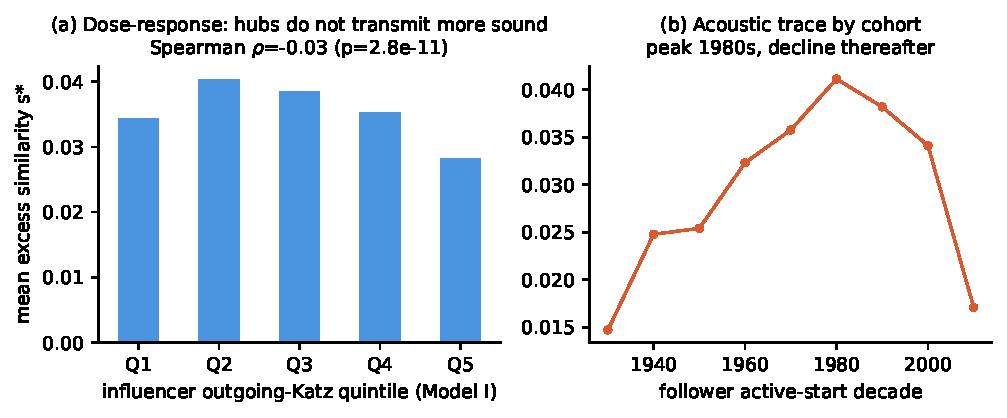
\includegraphics[width=0.95\textwidth]{dose_response_excess.pdf}
\caption{(a)~Mean excess similarity by influencer Katz quintile: the
acoustic trace \emph{weakens} for the most influential artists.
(b)~Mean excess similarity by follower active-start decade: the trace
rises to a 1980s peak ($0.041$) and falls sharply for the sparse 2010s
cohort ($n=798$).}
\label{fig:q4-dose}
\end{figure}

The decade curve (\cref{fig:q4-dose}, right) adds a temporal dimension
that connects to \cref{subsec:q3-inf-time}: the acoustic trace peaks for
followers starting in the 1980s ($0.041$) and collapses for the 2010s
cohort ($0.017$, $n=798$). Notably its peak lags the cross-genre flow
peak of \cref{subsec:q3-inf-time} (1960s) by two decades: the
\emph{breadth} of influence across genre boundaries narrowed first,
while the \emph{depth} of per-edge acoustic alignment kept rising into
the 1980s before falling---influence became narrower but more intense
before both declined.

\paragraph{Robustness and disclosure.}
The design inherits Assumption~A2 (active-start decade as the time
axis) and the cleaned edge table of section~4, including the $733$
time-reversed edges (A3); excluding them changes no conclusion because
the control construction does not depend on edge direction. The
\texttt{popularity} coordinate is retained for comparability with
Model~II, but its known within-year drift (section~5) makes its excess
($0.049$) hard to interpret, and it is excluded from the contagion
ranking. Raising the control count from $K=10$ to $K=25$ on a random
$4{,}000$-edge subsample changes $\bar{s}^{*}$ by $0.0004$. Two limitations bound the claims:
the data provide one acoustic snapshot per artist, so we cannot observe
change after the reported influence (hence ``consistent with'', not
``proves''), and influence not mediated by audio features (lyrics,
image, production practices) is invisible to this test.
